\section{Описание практической части}
\label{sec:Chapter4} \index{Chapter4}

Компилятор рассматриваемого языка в основном написан на языке программирования C++.

Для наглядности далее в тексте в качестве базового примера будут использоваться типы:
int (примитивный) → Int (объектный аналог)

\subsection{Арифметические операции}
На данном этапе работы было необходимо модифицировать проверку корректности типов в арифметческих операциях:
\begin{itemize}[label={}]
    \item \code{+} , \code{-} , \code{+=} , \code{-=}
    \item \code{++} , \code{--}
    \item \code{*} , \code{/} , \code{\%} , \code{*=}, \code{/=}, \code{\%=}
    \item \code{$\langle \langle$} , \code{$\rangle \rangle$} , \code{$\langle \langle$=} , \code{$\rangle \rangle$=}, \code{$\rangle \rangle \rangle$}, \code{$\rangle \rangle \rangle$=}
    \item \code{|} , \code{|=} , \code{\&} , \code{\&=}, \code{\^}, \code{\^}\code{=}, \code{||} , \code{\&\&}
    \item \code{<} , \code{<=} , \code{>}, \code{>=}, \code{==}, \code{===}, \code{!}
    \item Устранение дуализма типов (как в Java) и проблем упаковки (как в C\#)
\end{itemize}

В существующей реализации почти в каждой функции проверки производилось безусловное приведение типов операторов к примитивным, поэтому первым этапом работы было удаление или изменение кода, который приводил бы к замене объектных типов на их примитивные аналоги. Далее, основная функция, которая была нужна почти для всех вышеперечисленных операций(исключая логические и унарные) - функция, вычисляющая тип результата бинарного выражения. Ее поведение основывается на иерархии численных типов, оговоренной в спецификации.
Следующий этап заключался в очистке кода от попыток свернуть константы в функциях проверки, чтобы вынести все константные вычисления в отдельный модуль.

\subsection{Преобразования типов}
Для реализации проверки легальности преобразования объектных примитивоподобных типов можно было переиспользовать алгоритм, использовавшийся для проверки преобразований примитивных типов, добавив дополнительные проверки на отношения объектов (Union и Enum).
Структура функции для проверки корректности преобразования представлена на \ref{fig:cmp}
\begin{figure}[H]
    \centering
    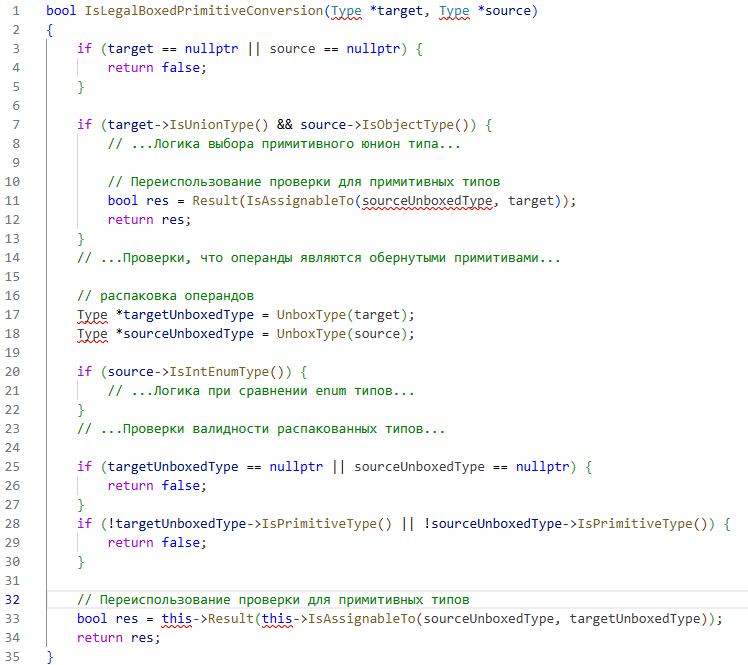
\includegraphics[scale=0.6]{image.png}
    \caption{Структура функции для проверки корректности преобразования примитивоподобных объектов}
    \label{fig:cmp}
\end{figure}

\subsection{Свёртка констант}
Один из основных этапов работы - это имплементация модуля компиляции для сверки констант в начало стадии семантического анализа.
Свёртка констант - вычисление константных выражений с последующей заменой выражений на результаты,
выполняемое на отдельной стадии компиляции. Это оптимизация, которая:
\begin{itemize}[label={--}]
    \item Ускоряет выполнение программы (избегает вычислений в runtime)
    \item Уменьшает размер генерируемого кода
    \item Позволяет обнаружить ошибки на этапе компиляции
\end{itemize}

Исплементированный модуль позволяет рекурсивно обойти const и readonly декларации и заменить константные выражения результатом их вычисления.
\subsubsection{Основной алгоритм}
\begin{enumerate}[label={--}]
    \item \textbf{Обход AST} - рекурсивных обход синтаксического дерева программы
    \item \textbf{Идентификация константных выражений} - проверка, можно ли вычислить выражение на этапе компиляции (является ли выражение константным)
    \item \textbf{Вычисление констант} - выполнение операций над константами
    \item \textbf{Замена выражений} - подстановка вычисленных значений вместо исходных выражений
\end{enumerate}

\subsubsection{Поддерживаемые типы и операции}
\textbf{Типы данных}
\begin{itemize}[label={--}]
    \item Числовые литералы (int, float, double)
    \item Символьные литералы (char)
    \item Булевы значения (true/false)
    \item Строковые литералы
    \item Enum значения
\end{itemize}

\textbf{Операции}
\begin{itemize}[label={--}]
    \item Арифметические  +, -, *, /, \%
    \item Битовые  \&, |, \^{}, \~{}, \verb|<<|, \verb|>>|, \verb|>>>|
    \item Логические  \&\&, ||, !
    \item Сравнения  ==, !=, <, >, <=, >=
    \item Унарные  +, -, \~{}
\end{itemize}

\subsubsection{Детали реализации}
\subsubsection*{Типизация и преобразование типов}
\begin{itemize}[label={--}]
    \item Используется система рангов типов TypeRank для определения приоритета преобразований
    \item Реализованы безопасные преобразования между типами с проверкой диапазонов
    \item Обработка деления на ноль
\end{itemize}

peremer

\subsubsection*{Обработка ошибок}
\begin{itemize}[label={--}]
    \item Генерация диагностических сообщений для недопустимых операций
    \item Реализованы безопасные преобразования между типами с проверкой диапазонов
    \item Отдельные функции преобразований между целыми и вещественными типами
\end{itemize}

\subsubsection*{Оптимизации}
\begin{itemize}[label={--}]
    \item Использование битовых операций для безопасной работы с целыми числами
    \item Специальная обработка строковых конкатенаций
    \item Оптимизация шаблонных литералов
\end{itemize}

\subsection{Оптимизация}
\newpage